\documentclass[11pt,a4paper]{article}

\usepackage{placeins}
\usepackage[a4paper,margin=2cm]{geometry}
\usepackage[T1]{fontenc}
\usepackage{enumitem}
\usepackage{hyperref}
\usepackage[dvipsnames]{xcolor}
\usepackage{amssymb}
\usepackage{wrapfig}
\usepackage{caption}
\usepackage[most]{tcolorbox}

\hypersetup{
    colorlinks=true,
    linkcolor=blue
}

\newcommand{\done}{{\color{Green}\Large\checkmark}}

\setlist{nosep}

\title{Structural Bioinformatics\\Oral Exam Preparation}
\author{}
\date{}

\begin{document}

\maketitle
\tableofcontents
\newpage

\section*{To do list (in order of importance)}:
\begin{enumerate}
\item SB08 Comparative Modelling \done
\item SB10 Ab Initio Methods \done
\item SB07 Evolution \done
\item SB06 Structural Alignments
\item SB04 Protein Folding \done
\item SB14 Molecular Dynamics
\item SB16 Embeddings
\item SB05 Structural Data \done
\item SB12-SB13 Disorder
\item SB09 Statistical Potentials
\item SB15 RING
\item SB11 Tandem Repeats
\item SB01-SB03 quick review
\end{enumerate}



\section*{Questions asked on the 24th June}
Open questions, quite broad.
\paragraph{Evolution}
\begin{enumerate}
    \item What is homology? 
    \item How do we understand if two proteins are homologous? (structure and sequence comparisons)
    \item What are the strategies and the databases that are used for classification of proteins? (Talk about SCOP, CATH, and their databases)
    \item Why does classification start from domains? What are they and why are they the important block?
\end{enumerate}

\paragraph{Structural alignment}
\begin{enumerate}
    \item What are the most effective strategies for alignment? 
    \item Talking about SSAP and TM-align specifically, what other algorithm do they remind you of? (dynamical programming for sequence alignment)
    \item How can you align two structures when their sequences don't have the same length?
    \item We talked about structural alignemnt. What is instead structural superposition? What is the minimization obiective that it is used?
\end{enumerate}


\paragraph{Protein Folding}
\begin{enumerate}
    \item Let's talk about the folding process
    \item What determines the stability of a protein?
    \item What happens if a protein misfolds? What are chaperones and what do they do?
\end{enumerate}

\section*{Course Recap - last lecture}
List of topics professor considers most important:
\vspace*{0.5em}
\begin{itemize}
    \item Knowing the difference between structural alignment and structural superposition
    \item Knowing how the Kabsch algorithm works for structural superposition
    \item Knowing what is a contact map and how to recognize alpha helices and beta sheets from it
    \item Remembering that we saw four different algorithms for structural alignment, and that they use different strategies and they may complement each other.
    \item Remembering the sequence-structure relationship: proteins can have similar structure but very low sequence identity. But viceversa, there is a threshold in sequence identity upon which
    we can be sure that the structures are similar. This threshold is 30\% sequence identity, which is not so high! That's why you can successfully do homology modelling. You dont need to have a very high sequence identity to be able to model a protein structure from a template.
    \item Knowing that we reconstruct the tree of life using protein sequence databases. Mutations are a "biological clock" that we can use to understand how long ago two animal species diverged from a common ancestor. The more similar the sequences we see in them today, the more recently they diverged. 
    \item Knowing that we infer homology \textbf{from sequence similarity}.
    \item We talked about understanding what is the "complement of folds" in nature, and how much the complement is shared across species. 
    \item the hypotesis of the universal common ancestor, and how this hypotesis is supported by structural data (complex proteins could result from the combination of simpler elements, and these simpler elements are shared across species)
    \item That the way we sytematically reason about complexity of protein structure across species is through \textbf{domain} classification.
    \item That domain are autonomous folding units, and that there is evidence that they evolved independently.
    \item Homologous and analogous are distinguished by looking at the sequence identity: if high, then homologous, if low, then analogous.
    \item SCOP and CATH are two different classification systems for protein domains.
    \item That homology modelling exploits the fact that upon $30\%$ sequence identity, we can be sure that the structures are similar. 
    \item That the scoring function of CASP is GDT (=Global Distance Test), which is a measure of how many residues are within a certain distance threshold from the native structure.
    \item The smart idea of Rosetta is that while for sure not every protein sequence is represented in the PDB, if we only consider short fragments ($9$ residues), then we can be sure that every possible fragment is represented in the PDB, and in many conformations.
    \item that rosetta uses discriminarory functions (statistical potentials) and simulated annealing.
\end{itemize}
\vspace*{0.5em}
That above is the core of the course. Then we covered a series of more specific and less technical topics: non globular proteins, disorder prediction, molecular dynamics, embeddings. Most important points:
\vspace*{0.5em}
\begin{itemize}
    \item There are proteins which dont assume a fixed structure (IDP - intrinsically disordered). they are designed to be like that.
    \item tandem repeats offer an extended platform for protein-protein interactions and they are used for designing new proteins with specific functions. Because you have a stable scaffold and you can make small mutations or indels and still get a protein that is able to folds and is stable.
    \item that tandem repeat proteins fold from one end to the other.
    \item we saw algorithms for detection of repeats in protein sequences (REPETITA, which exploits Atchley scales, RAPHAEL, and dot plots).
    \item Embeddings.
\end{itemize}
%%%%%%%%%%%%%%%%%%%%%%%%%%%%%%%%%%%%%%%%%%%%%%%%%%%%%%%%%%%%
\section{SB01 -- Introduction to Structural Bioinformatics}

\subsection*{Table of Contents}
\begin{enumerate}
\item Definition of bioinformatics
\item Structural bioinformatics
\item Central dogma of molecular biology
\item Protein structure and function
\item Structure prediction problem
\item Sequence--structure gap
\item Protein folding problem
\item AlphaFold and AI-based prediction
\item Course objectives
\item Computational tools and applications
\end{enumerate}


\subsection*{Possible questions:}
\begin{enumerate}
\item{What is structural bioinformatics?}
\item{How does structural bioinformatics differ from classical bioinformatics?}
\item{What is the sequence--structure gap?}
\item{Why is protein structure important for understanding function?}
\item{What is the protein folding problem?}
\item{Why was protein structure prediction historically difficult?}
\item{How did AlphaFold change the field?}
\item{What disciplines contribute to bioinformatics?}
\item{What are the main applications of structural bioinformatics?}
\item{What computational skills are important in this field?}
\end{enumerate}
\section{SB02 -- Chemical Bonds}

\subsection*{Table of Contents}
\begin{enumerate}
\item Matter and chemical transformations
\item Atomic theory
\item Atomic structure
\item Electrons and orbitals
\item Chemical bonding principles
\item Covalent bonds
\item Ionic interactions
\item Electronegativity
\item Molecular geometry
\item Non-covalent interactions in biomolecules
\end{enumerate}

\subsection*{Possible questions:}
\begin{enumerate}
\item{What is the difference between physical and chemical transformations?}
\item{Describe the structure of an atom.}
\item{What are orbitals and quantum numbers?}
\item{Explain the Aufbau principle.}
\item{What is electronegativity?}
\item{Compare covalent and ionic bonds.}
\item{What determines bond polarity?}
\item{Why are non-covalent interactions important in proteins?}
\item{What role do hydrogen bonds play in biology?}
\item{Why is carbon particularly suited for life?}
\end{enumerate}
\section{SB03 -- Amino Acids / Acid-Base Theory}

\subsection*{Table of Contents}
\begin{enumerate}
\item Arrhenius theory
\item Br{\o}nsted--Lowry theory
\item Acids and bases in aqueous solution
\item Strong vs weak acids
\item Acid dissociation constant
\item pKa
\item pH and pOH
\item Water self-ionization
\item Amino acid ionization
\item Buffer systems
\end{enumerate}

\subsection*{Possible questions:}
\begin{enumerate}
\item{Compare Arrhenius and Br{\o}nsted--Lowry theories.}
\item{What is a conjugate acid-base pair?}
\item{Define Ka and pKa.}
\item{What is the relationship between pKa and acid strength?}
\item{What is the difference between a strong acid and a weak acid?}
\item{What is the significance of pH?}
\item{Why is water amphoteric?}
\item{What is a buffer?}
\item{Explain the Henderson--Hasselbalch equation.}
\item{How do amino acids behave at different pH values?}
\item{What is the isoelectric point of a protein?}
\end{enumerate}
\section{SB04 -- Protein Folding}

\subsection*{Table of Contents}
\begin{enumerate}
\item Protein folding problem
\item Native and denatured states
\item Levinthal's paradox
\item Secondary structure
\item Folding pathways
\item Energy landscape
\item Thermodynamics of folding
\item Folding kinetics
\item Chaperones
\item Misfolding and aggregation
\end{enumerate}

\subsection*{Possible questions:}
\begin{enumerate}
\item{\textcolor{blue}{What is the native state of a protein?}}
\item{What is the protein folding problem?}
\item{What is the typical folding timescale in biological proteins?}
\item{What is Levinthal's paradox?}
\item{What are the main secondary structures?}
\item {What are the backbone dihedral angles?}
\item {What is the Ramachandran plot?}
\item {How can we describe the folding process in terms variations of thermodynamic variables?}
\item{What is the hydrophobic effect?}
\item{What stabilizes the native state?}
\item{Difference between thermodynamics and kinetics of folding?}
\item{Why is protein folding not a random search?}
\item{Explain the energy funnel model.}
\item {What is the principle of minimal frustration?}
\item {What is residual frustration and why is it important?}
\item{What are molecular chaperones?}
\item{How is misfolding related to disease?}
\end{enumerate}

\newpage

\paragraph{What is the protein folding problem?}
Most proteins in biological systems are functional only when they are folded into a specific 3D structure, called the native state. The process by which a protein acquires its native structure is called folding. The protein folding problem is the challenge of understanding both \textbf{which} is the 3d structure that the protein will fold into (the native structure) starting from the sequence, and \textbf{how}
it will get there, meaning which sequence of conformations will it sample, and if there is a specific, dominant pathway that it will follow, or many.


So the protein folding problem has mainly two parts: one is the \textbf{structure prediction problem}, which is the question that methods like AlphFold are trying to answer,
and the other is the \textbf{folding mechanism problem}, which is the question of how the protein gets to its native state, and regards the kinetics of folding.

The structure prediction problem is framed like this: given the aminoacid sequence, find the \textbf{injective function} that maps the sequence to the 3D structure. 
Methods like alphafold try to learn this function from the data, and they are very successful at it. However, they do not give us any insight into the folding mechanism problem, which is still an open question.
Also, these methods are instrinsically limited by the data they are trained on: for instance, they only predict with a water environment, cannot say anything about what happens when the protein 
is in a different solvent, and they saw only the 20 L-aminoacids in the training data, so they cannot predict what happens when there are post-translational modifications, or non-natural aminoacids.


\paragraph{What is the typical folding timescale in biological proteins?}
Most biological proteins fold spontaneously on timescales ranging from microseconds to seconds, although the exact folding rate depends on protein size, topology, and stability. Small single-domain proteins can fold in microseconds or milliseconds, whereas larger proteins may require seconds or the assistance of molecular chaperones.


\paragraph{What is Levinthal's paradox?}

Levinthal's paradox is the observation that proteins fold into their native structure much faster than would be possible if they explored all possible conformations randomly. Cyrus Levinthal estimated that even a small protein could adopt an astronomically large number of conformations, making a random search of conformational space effectively impossible within the age of the universe.
However, experimental observations show that most proteins fold in times ranging from microseconds to seconds. This apparent contradiction suggests that protein folding is not a random search process. Instead, proteins fold through biased pathways guided by an energy landscape that directs the molecule toward the native state.
Additionally, biological proteins are not random sequences, but have been selected through evolution to fold in timescales compatible with life.

\paragraph{What are the main secondary structures?}
Secondary structure refers to local, regularly recurring arrangements of the protein backbone \textbf{stabilized primarily by hydrogen bonds} between backbone amide and carbonyl groups. The two most common secondary structures are the $\alpha$-helix and the $\beta$-sheet.
An $\alpha$-helix is a right-handed helical structure in which each carbonyl oxygen forms a hydrogen bond with the amide hydrogen four residues ahead in the sequence ($i \rightarrow i+4$). A $\beta$-sheet consists of extended $\beta$-strands connected by hydrogen bonds and can be either parallel or antiparallel. The antiparallel arrangement
is the most stable because it allows atoms that participate in the hydrogen bond to get closer.

\paragraph{What are the backbone dihedral angles?}
\begin{center}
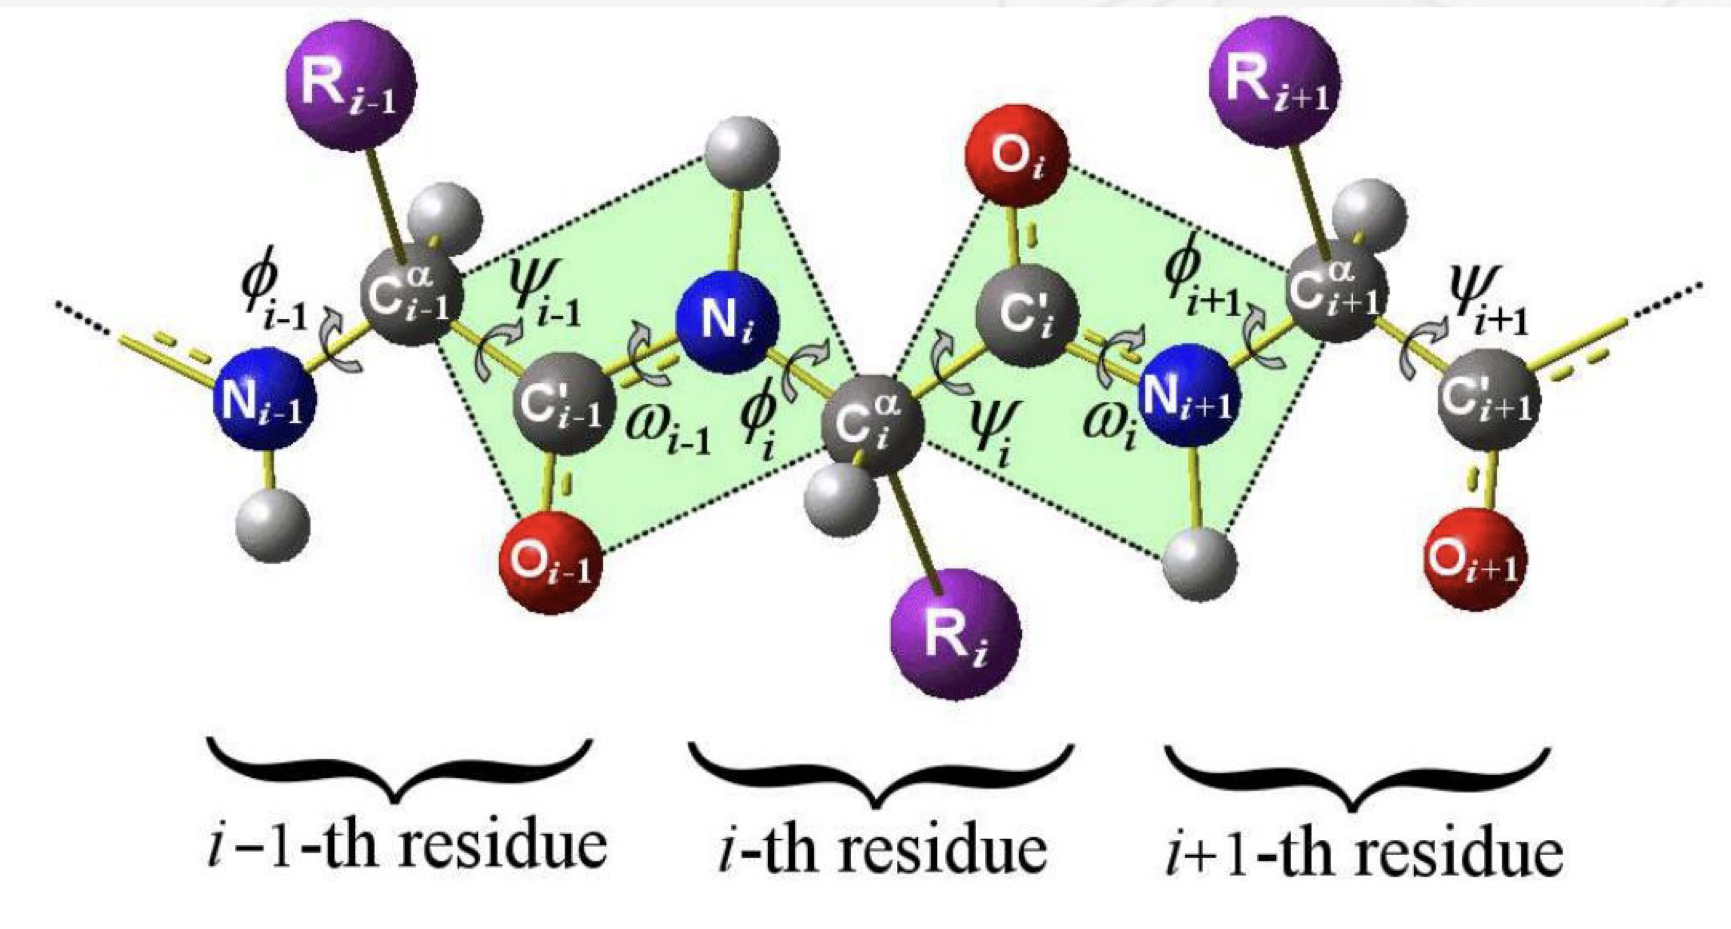
\includegraphics[width=0.5\textwidth]{figures/dihedrals.png}
\end{center}
The bond $N-C_\alpha - C_{\beta}$ is rigid and planar. Therefore, the backbone conformation of a protein can be described by two dihedral angles: $\phi$ (phi) and $\psi$ (psi). The $\phi$ angle is the rotation around the N-$C_\alpha$ bond and is defined by the three atoms ($C_{\beta}^{-1}, N,C_{\alpha}$), while the $\psi$ angle is the rotation around the $C_\alpha - C_{\beta}$ bond
and is defined by the three atoms ($C_{\alpha}, C_{\beta}, N^{+1}$). 

\paragraph{What is the Ramachandran plot?}
The Ramachandran plot is a graphical representation of the backbone dihedral angles $\phi$ and $\psi$ . Each point on the plot corresponds to a particular combination of these two angles, allowing visualization of the conformational space accessible to the protein backbone.
Because of steric repulsion between atoms, many combinations of $\phi$ and $\psi$ are energetically unfavorable and therefore forbidden. As a result, residues cluster in a few allowed regions corresponding to common secondary structures. For example, right-handed $\alpha$-helices and $\beta$-sheets occupy distinct areas of the Ramachandran plot.
The Ramachandran plot is widely used to understand protein structure and to assess the quality of experimentally determined or predicted structures. A high-quality protein model should have most residues located in energetically allowed regions, while residues in disallowed regions may indicate structural errors or unusual conformations.


\paragraph{How can we describe the folding process in terms of variations of thermodynamic variables?}

Protein folding can be described using the Gibbs free energy change

\[
\Delta G_{fold} = \Delta H_{fold} - T\Delta S_{fold}.
\]

Folding is thermodynamically favorable when $\Delta G_{fold}<0$, meaning that the folded state has a lower free energy than the unfolded state. The enthalpy term $\Delta H_{fold}$ is generally negative because folding creates stabilizing interactions such as hydrogen bonds, van der Waals contacts, and salt bridges.

The entropy change has two opposing contributions:

\[
\Delta S_{fold} = \Delta S_{conf} + \Delta S_{solvent}
\]

The protein loses conformational freedom upon folding, leading to a decrease in conformational entropy ($\Delta S_{conf}<0$), which opposes folding. However, hydrophobic residues become buried in the protein core, releasing ordered water molecules into the solvent and increasing solvent entropy ($\Delta S_{solvent}>0$), which favors folding.

Overall, the sign of $\Delta G_{fold}$ depends on the balance between these enthalpic and entropic contributions. Usually it is negative, meaning that the folded state is thermodynamically favored. But not by a lot: it is said that proteins are "marginally stable": the free energy difference between the folded and unfolded states is typically only a few kcal/mol ($5-15$), which is 
small compared to the total energy of the protein (for a comparison, a single hydrogen bond acocunts for $1-5\, kcal/mol$). This marginal stability allows proteins to be flexible and dynamic, enabling them to perform their biological functions effectively.


\paragraph{What is the hydrophobic effect?}
The hydrophobic effect is the tendency of nonpolar molecules or side chains to cluster together in aqueous environments. In proteins, hydrophobic residues such as Val, Leu, Ile, Phe, and Met are typically buried in the protein core, while polar and charged residues remain exposed to the solvent.
The driving force behind the hydrophobic effect is not a direct attraction between hydrophobic groups. Instead, it arises from the behavior of water molecules. When hydrophobic residues are exposed, surrounding water molecules become highly ordered to maintain their hydrogen-bonding network. This ordering decreases the entropy of the solvent. Upon folding, hydrophobic residues are buried, reducing the exposed hydrophobic surface and releasing these ordered water molecules into the bulk solvent, thereby increasing solvent entropy.
The hydrophobic effect is one of the major driving forces of protein folding. 


\paragraph{Why is protein folding not a random search?}
Because it cannot be. The Levital's paradox assumed that every residue can sample all possible conformations independently. But this is not true, there are constraints on the conformational space that the protein can sample, such as steric hindrance and the formation of local secondary structures. These constraints significantly reduce the number of conformations that need to be explored.
Also, the folding process is guided by an energy landscape that directs the protein towards the native state. As some of the native interaction form, the space of possibilities gets restricted and 
other native interactions become more likely to form, and this goes on till the protein reaches the minimum of the energy landscape, which is the native state. 





\paragraph{Explain the energy funnel model view and how it differs from the ant trail view}
The funnel model essentially says that at the start of the folding process, the protein can sample a wide variety of conformations, but as it folds and forms native interactions, the conformational space narrows down. 
This is a funnel-shaped energy landscape, where the bottom represents the native state. The folding process is stochastic: usually there is no "single" pathway dominating over the others.
Different molecules of the same protein may follow different routes and visit different intermediates, yet still reach the same native structure.



\paragraph{What is the principle of minimal frustration?}

Frustration means that different interactions “disagree” about what the structure should be. Minimal frustration means that most interactions “agree” that the native state is the best solution.
This concept is tightly connected to the energy funnel model: the funnel exists precisely because evolution has minimized frustration in naturally occurring protein sequences.


The principle of minimal frustration states that natural proteins have evolved sequences in which most interactions favor the formation of the native structure rather than competing with it. As a result, the energy landscape is biased toward the native state and contains relatively few energetic conflicts, or \emph{frustrations}, that could trap the protein in incorrect conformations. It is
overall a quite smooth landscape. This greatly reduces the number of kinetic traps and allows proteins to fold rapidly and reproducibly.


\paragraph{What is residual frustration and why is it important?}

Although natural proteins obey the principle of minimal frustration, frustration is not completely eliminated. \emph{Residual frustration} refers to the small number of interactions within a folded protein that are not fully optimized for structural stability and that locally favor alternative conformations or competing interactions.
Residual frustration is important because proteins are not evolved solely for stability. Many functional processes, such as ligand binding, allosteric regulation, conformational changes, and enzymatic catalysis, require a certain degree of flexibility and structural adaptability. Locally frustrated regions often coincide with active sites, binding interfaces, or regions involved in molecular recognition.
Therefore, while minimal frustration enables efficient folding by creating a funnel-shaped energy landscape, residual frustration provides the flexibility necessary for biological function. Proteins can be viewed as a compromise between the requirements of stability and the requirements of activity.

\paragraph{How is misfolding related to disease?}

Protein misfolding occurs when a protein fails to reach its native structure or adopts an alternative conformation that is unstable or non-functional. Misfolded proteins may lose their biological activity, become degraded, or aggregate with other misfolded molecules. Because protein function depends strongly on structure, misfolding can have severe cellular consequences.
Many diseases are associated with the accumulation of misfolded proteins and the formation of insoluble aggregates or amyloid fibrils. Examples include Alzheimer's disease, which involves aggregation of amyloid-$\beta$ peptides; Parkinson's disease, associated with $\alpha$-synuclein aggregates; and prion diseases, in which a misfolded protein induces the misfolding of other copies of the same protein. In these cases, protein aggregation can disrupt cellular processes and lead to cell death.
Cells possess quality-control mechanisms, including molecular chaperones and degradation pathways, that help proteins fold correctly and remove misfolded species. Disease can arise when these systems are overwhelmed or when mutations increase the tendency of a protein to misfold and aggregate.
\section{SB05 -- Structural Data}

\subsection*{Table of Contents}

\begin{enumerate}
\item Experimental determination of protein structures
\item X-ray crystallography
\item Nuclear Magnetic Resonance (NMR)
\item Cryo-Electron Microscopy (Cryo-EM)
\item Protein Data Bank (PDB)
\item PDB file formats and annotations
\item Structure quality and resolution
\item Biological assemblies and complexes
\item Structural databases and resources
\item Applications of structural data
\end{enumerate}


\subsection*{Possible questions:}
\begin{enumerate}
\item{What is the Protein Data Bank (PDB)?}
\item{Which information is contained in a PDB structure file?}
\item{What experimental techniques are used to determine protein structures?}
\item{What is the difference between X-ray crystallography, NMR spectroscopy and cryo-EM?}
\item{What is meant by resolution in structural biology?}
\item{What is a biological assembly and how does it differ from the asymmetric unit?}
\item{What are "missing residues" in a PDB structure and why do they occur?}
\item{Why is structural annotation important?}
\item{What are PDB-derived databases and why are they useful?}
\item{How can structural data contribute to drug discovery and protein engineering?}
\item{What are the main limitations and biases of currently available structural datasets?}

% Optional integrative questions

\item{How has the growth of the PDB enabled the development of comparative modelling and AlphaFold?}
\item{Why is structure determination still important despite highly accurate structure prediction methods?}
\item{How are experimental structures used to derive statistical potentials and train machine learning models?}
\end{enumerate}
%%%%%%%%%%%%%%%%%%%%%%%%%%%%%%%%%%%%%%%%%%%%%%%%%%%%%%%%%%%%
\section{SB06 -- Structural Alignments}

\subsection*{Table of Contents}

\begin{enumerate}
\item Structural comparison of proteins
\item Structural superposition
\item Protein structure representations
\item Root Mean Square Deviation (RMSD)
\item Kabsch algorithm
\item Global and local structural alignment
\item Alignment scoring and significance
\item Structural similarity measures
\item Conservation of structure versus sequence
\item Applications of structural alignments
\end{enumerate}


\begin{enumerate}
\item{What is RMSD?}
\item{How is RMSD calculated?}
\item{What is the difference between structural alignment and structural superposition?}
\item{What is the Kabsch algorithm?}
\item{Why are structural alignments more difficult than sequence alignments?}
\item{What information is lost when using only C$\alpha$ atoms?}
\item{What are equivalent residues in a structural alignment?}
\item{Why can structure be more conserved than sequence?}
\item{What are the limitations of RMSD as a similarity measure?}
\item{When is structural comparison useful in bioinformatics?}
\end{enumerate}
%%%%%%%%%%%%%%%%%%%%%%%%%%%%%%%%%%%%%%%%%%%%%%%%%%%%%%%%%%%%
\section{SB07 -- Structural Evolution}

\subsection*{Table of Contents}

\begin{enumerate}
\item Protein evolution
\item Sequence-structure relationship
\item Structural conservation
\item Homology and analogy
\item Divergent evolution
\item Convergent evolution
\item Protein folds and fold space
\item Structural classification systems
\item Remote homology detection
\item Evolutionary constraints on protein structure
\end{enumerate}

\begin{enumerate}
\item{Why is protein structure generally more conserved than sequence?}
\item{What is the relation between sequence similarity and structural similarity in biological proteins?}
\item{What level of sequence identity is usually associated with structural similarity?}
\item{What are homologous proteins?}
\item{What is divergent evolution?}
\item{What is convergent evolution?}
\item{Can proteins with low sequence identity have similar structures?}
\item{What is a protein fold?}
\item{Explain the Rossmann fold as an example of structural conservation.}
\item{How does evolution constrain protein structure?}
\item{Why is structural information useful for detecting remote homology?}
\end{enumerate}
%%%%%%%%%%%%%%%%%%%%%%%%%%%%%%%%%%%%%%%%%%%%%%%%%%%%%%%%%%%%
\section{SB08 -- Comparative (Homology) Modelling \done}

\subsection*{Table of Contents}

\begin{enumerate}
\item Protein structure prediction
\item Principles of homology modelling
\item Template identification
\item Sequence alignment
\item Model building
\item Loop modelling
\item Side-chain modelling
\item Model refinement
\item Model validation and quality assessment
\item Limitations of comparative modelling
\end{enumerate}


\subsection*{Possible Exam Questions:}

\begin{enumerate}
\item{\textcolor{blue}{Describe the main steps involved in homology (comparative) modelling.} \done}
\item{Why is sequence alignment the most critical step? \done}
\item{Explain the difference between \textit{fragment-based} and \textit{restraint-based} raw model building. \done}
\item{How are side chains modelled? \done}
\item{How is model quality evaluated? \done}
\item{What are the main limitations of comparative modelling? \done}
\end{enumerate}


\paragraph{Describe the main steps involved in homology (comparative) modelling.}
Homology modelling is the method of predicting the structure of a protein (“target”) based on
experimentally determined structures of other proteins (“templates”). Main steps:

\begin{enumerate}
\item template identification: search databases for homologous proteins with known
structures;
\item sequence alignment: align target and template. 
\item building raw model: for aligned regions, backbone coordinates of the template are
directly copied to the target model;
\item loop modelling: coordinates for the variable regions (e.g. loops) and positions near
indels must be predicted.
\item side chains refinement: the side chains of the target sequence are added to the
backbone model, and their positioning is optimised to reduce steric clashes;
\item model plausibility assessment: stereochemical checks (e.g. bond lengths, angles,
Ramachandran plot), detection of steric clashes, computation of knowledge-based
scoring functions (statistical potentials) for comparison with experimentally observed
structures.
\end{enumerate}

\paragraph{Why is sequence alignment the most critical step in the homology modelling pipeline?}
Often, the best sequence alignment (the one that maximizes alignment score) is not optimal for structure modelling. Suboptimal choices at this stage cannot be corrected in the following steps. This makes the sequence alignment the most critical step in homology modelling.


\paragraph{Explain the difference between fragment-based and restraint-based raw model building.}
In comparative modelling, once the target-template alignment has been obtained, the raw model can be built using different strategies.

\noindent In fragment-based building, useful structural fragments are directly copied from one or more templates and assembled into the target model. The main advantage is that the copied fragments already have realistic local geometry, so important regions such as an active site can be preserved accurately. However, different fragments must then be joined together, and this may create problems in the global consistency of the model.

\noindent In restraint-based building, instead of copying entire fragments, the template is used to derive geometrical restraints on the target structure, for example approximate atomic positions, distances, or angles. The model is then obtained by optimizing the structure so that these restraints are satisfied as well as possible. This produces a globally optimized structure and spreads errors over the whole model, but it does not necessarily preserve the exact local geometry of specific functional regions.

\paragraph{How are side chains modelled?}

Side chains are usually modelled after the backbone has been constructed. Their conformations are mainly determined by rotations around single bonds, described by the side-chain torsion angles $\chi$. These angles do not take arbitrary values, but tend to adopt a small number of preferred conformations called \textbf{rotamers}. For each torsion angle, the main preferred positions are:
gauche$^+$, around $60^\circ$, gauche$^-$, around $-60^\circ$, and trans, around $180^\circ$.
\begin{center}
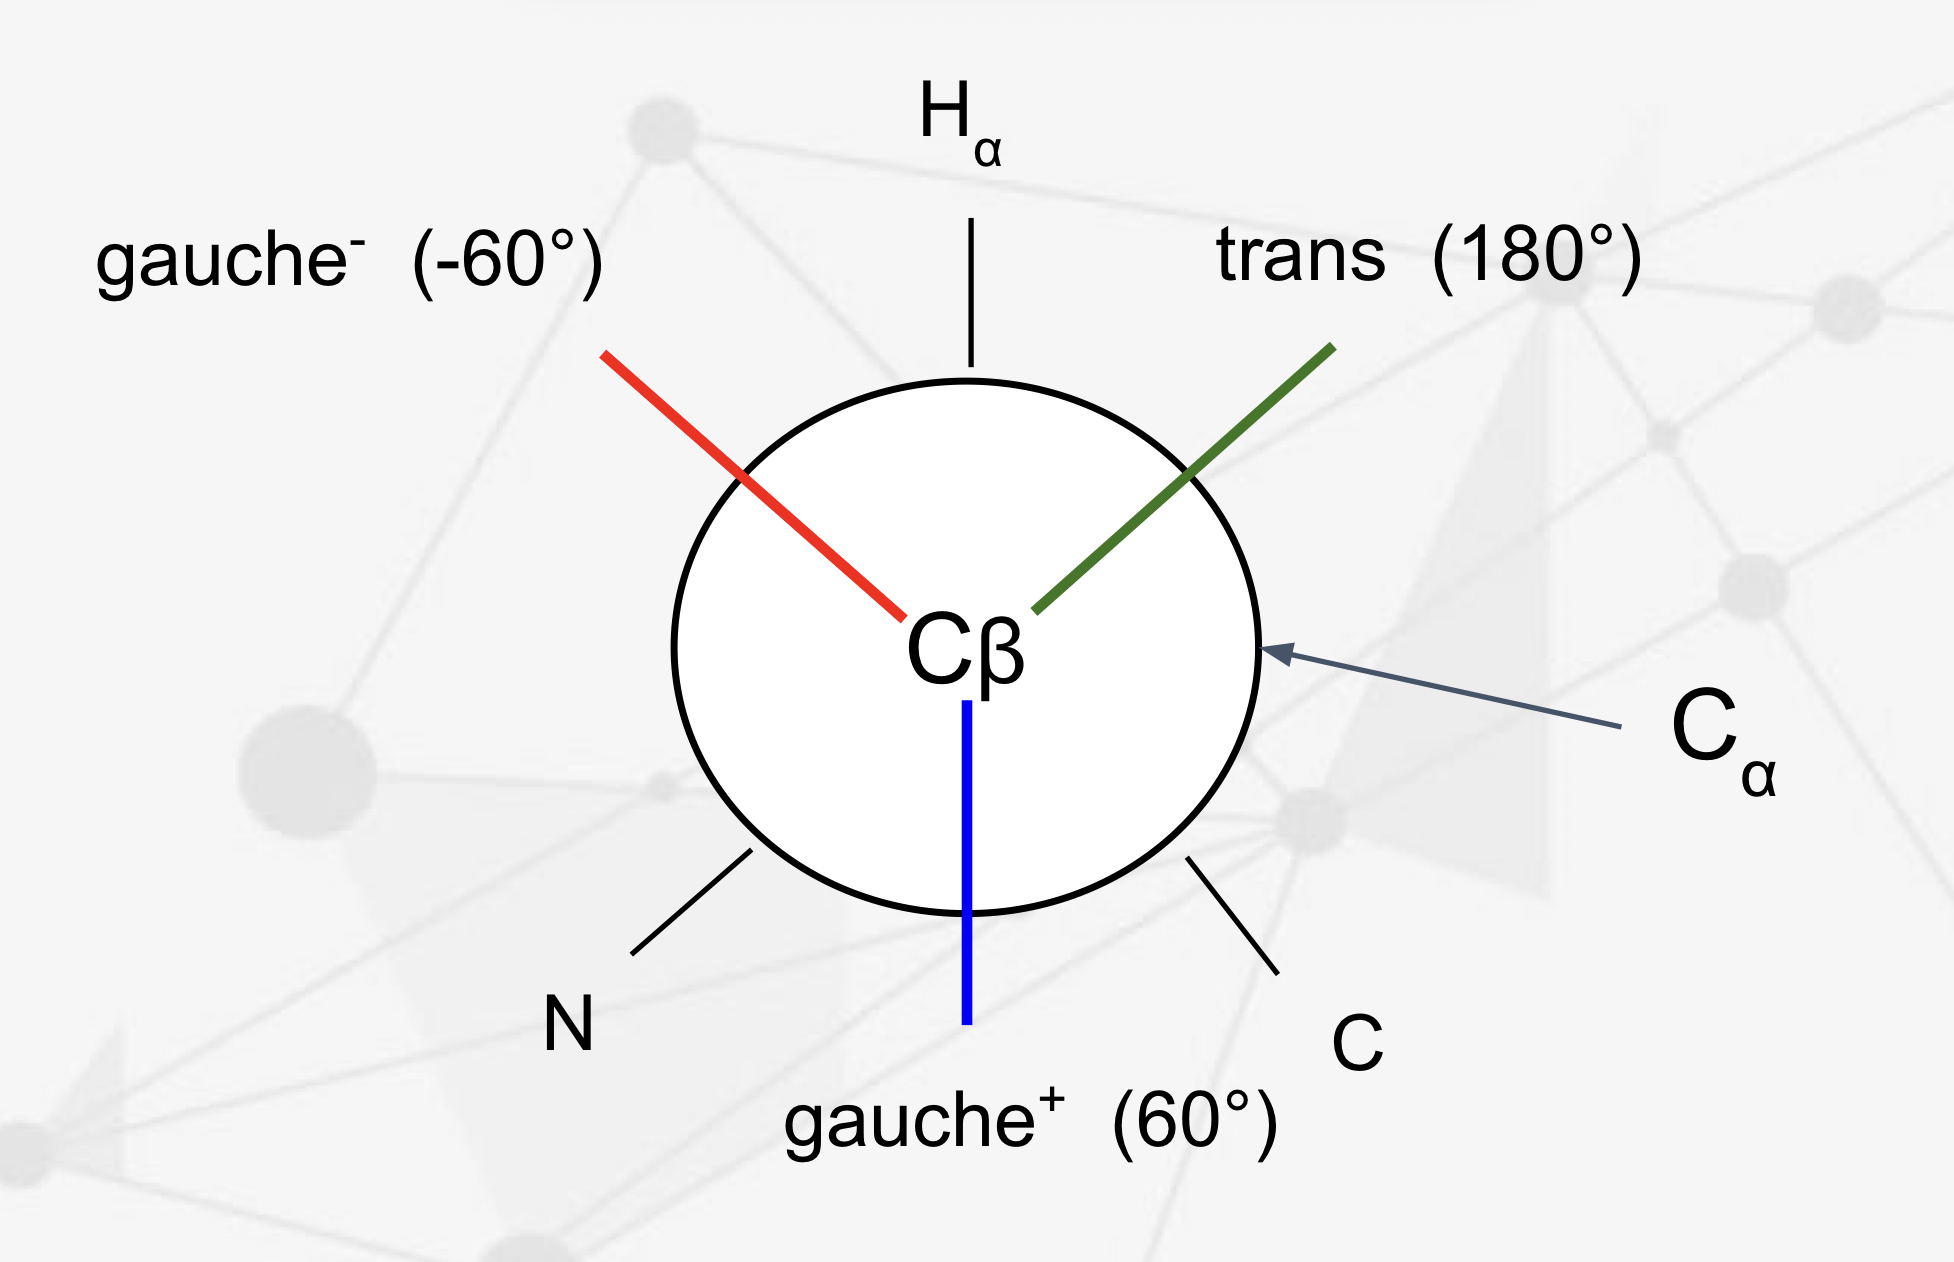
\includegraphics[width=0.4\textwidth]{figures/rotameters.png}
\end{center}
In homology modelling, side chains are therefore modelled by choosing suitable rotamers from a rotamer library. The probability of each rotamer depends on the type of amino acid and on the local backbone conformation, especially the backbone torsion angles $\phi$ and $\psi$. Side-chain modelling is not independent residue by residue, because the conformation chosen for one side chain can affect neighbouring residues through steric clashes and packing interactions. This creates a domino effect. When possible, it is preferable to keep the conformation of the template side chains, especially in conserved or functionally important regions, because they may already represent a realistic local geometry.

\paragraph{How is model quality assessed?}
The quality of a homology model is assessed by checking both its stereochemical correctness and its compatibility with known protein structures. First, one looks for \textbf{steric clashes}, where atoms are unrealistically close to each other. A good model should not contain severe overlaps between atoms. Second, one checks the \textbf{standard geometry} of the model, such as bond lengths, bond angles, peptide planarity, and backbone torsion angles. For example, the $\phi$ and $\psi$ angles should mostly fall in allowed regions of the Ramachandran plot.

A further level of assessment uses \textbf{statistical potentials} or frequency profiles. These methods compare the local environment of each residue with what is commonly observed in experimentally solved protein structures. For example, hydrophobic residues are expected to be buried, polar residues are often exposed, and certain residue types prefer specific secondary-structure or packing environments. If many residues are found in unusual environments, this suggests that the model may be unreliable.


\paragraph{What are the main limitations of comparative modelling?}
The main limitations of comparative modelling are i) the fact that the model will be more precise in regions that are conserved between the target and the template, and less accurate in variable regions such as loops; ii) that
you need homologous templates with known structures, which may not be available for all target sequences. In fact, $40\%$ of known genes are not homologous to known structures. This strongly limits the applicability  of homology modelling.
%%%%%%%%%%%%%%%%%%%%%%%%%%%%%%%%%%%%%%%%%%%%%%%%%%%%%%%%%%%%
\section{SB09 -- Statistical Potentials}

\subsection*{Table of Contents}

\begin{enumerate}
\item Protein scoring functions
\item Native versus non-native structures
\item Knowledge-based potentials
\item Distance-dependent statistical potentials
\item RAPDF
\item Bayesian formulation
\item Likelihood and prior probabilities
\item Structure evaluation
\item Fold recognition
\item Advantages and limitations of statistical potentials
\end{enumerate}

\begin{enumerate}
\item{What is a statistical potential?}
\item{How are statistical potentials derived from structural databases?}
\item{What is RAPDF?}
\item{Why are native structures distinguishable from non-native structures?}
\item{What is the role of Bayes' theorem in statistical potentials?}
\item{What assumptions underlie RAPDF?}
\item{How are residue-residue distances used in scoring functions?}
\item{What is the difference between physical and statistical potentials?}
\item{What applications do statistical potentials have in structural bioinformatics?}
\item{What are the main limitations of statistical potentials?}
\end{enumerate}
%%%%%%%%%%%%%%%%%%%%%%%%%%%%%%%%%%%%%%%%%%%%%%%%%%%%%%%%%%%%
\section{SB10 -- Ab Initio Methods}

\subsection*{Table of Contents}

\begin{enumerate}
\item CASP experiments
\item Categories of structure prediction methods
\item Template-free prediction
\item Fragment assembly methods
\item Conformational search
\item Energy functions
\item Sampling strategies
\item Prediction assessment
\item AlphaFold and deep learning approaches
\item Current challenges and future directions
\end{enumerate}


\begin{enumerate}
\item{What is CASP and why is it important?}
\item{What does the term 'ab initio prediction' mean?}
\item{What is the difference between template-based and template-free prediction?}
\item{How does fragment assembly work?}
\item{Why are ab initio methods computationally expensive?}
\item{What role do energy functions play in structure prediction?}
\item{How is conformational space explored in ab initio prediction?}
\item{How are predicted structures evaluated?}
\item{How did AlphaFold change the field of structure prediction?}
\item{What challenges remain in protein structure prediction?}
\end{enumerate}
%%%%%%%%%%%%%%%%%%%%%%%%%%%%%%%%%%%%%%%%%%%%%%%%%%%%%%%%%%%%
\section{SB11 -- Tandem Repeat Proteins}

\subsection*{Table of Contents}

\begin{enumerate}
\item Tandem repeat proteins
\item Structural organization of repeats
\item Repeat unit identification
\item Evolution through duplication
\item Structural symmetry
\item Functional roles of repeat proteins
\item Hydrophobicity and sequence patterns
\item Repeat classification
\item RepeatsDB
\item Disease-related repeat proteins
\end{enumerate}


\begin{enumerate}
\item{What is a tandem repeat protein?}
\item{How do tandem repeats arise during evolution?}
\item{Why are tandem repeat proteins particularly common in eukaryotes?}
\item{What biological functions are associated with repeat proteins?}
\item{How can tandem repeats be identified from sequence or structure?}
\item{What is structural symmetry in repeat proteins?}
\item{Why do repeat proteins evolve rapidly?}
\item{How are tandem repeats associated with disease?}
\item{What is RepeatsDB and what information does it provide?}
\item{How do tandem repeat proteins differ from globular proteins?}
\end{enumerate}
%%%%%%%%%%%%%%%%%%%%%%%%%%%%%%%%%%%%%%%%%%%%%%%%%%%%%%%%%%%%
\section{SB12 -- Intrinsically Disordered Proteins}

\subsection*{Table of Contents}

\begin{enumerate}
\item Definition of intrinsically disordered proteins
\item Historical perspective
\item Structural disorder versus ordered proteins
\item Functional roles of disorder
\item Coupled folding and binding
\item Induced fit mechanisms
\item Signalling and regulation
\item Protein interaction networks
\item Experimental characterization of IDPs
\item Biological significance of disorder
\end{enumerate}


\begin{enumerate}
\item{What is an intrinsically disordered protein (IDP)?}
\item{Why can proteins lacking a stable structure still be functional?}
\item{What is coupled folding and binding?}
\item{What is induced fit?}
\item{Why are IDPs frequently involved in signalling and regulation?}
\item{Which sequence features are characteristic of IDPs?}
\item{How do IDPs differ from globular proteins in terms of aminoacid composition?}
\item{What advantages does structural disorder provide?}
\item{Why are intrinsically disordered proteins difficult to study experimentally?}
\item{Give examples of biological functions performed by IDPs.}
\end{enumerate}
%%%%%%%%%%%%%%%%%%%%%%%%%%%%%%%%%%%%%%%%%%%%%%%%%%%%%%%%%%%%
\section{SB13 -- Disorder Prediction}

\subsection*{Table of Contents}

\begin{enumerate}
\item Low-complexity regions
\item SEG algorithm
\item NORS proteins
\item Amino-acid composition of disordered regions
\item Charge and hydrophobicity
\item Compositional bias
\item Evolution of intrinsic disorder
\item Sequence-based prediction methods
\item Benchmarking and CAID
\item Applications of disorder prediction
\end{enumerate}

\begin{enumerate}
\item{What are low-complexity regions?}
\item{How does the SEG algorithm identify low-complexity regions?}
\item{What are NORS proteins?}
\item{Which amino acids are enriched in intrinsically disordered regions?}
\item{Why are hydrophobic residues generally depleted in disordered proteins?}
\item{How does net charge contribute to disorder?}
\item{What is compositional bias?}
\item{Why is intrinsic disorder more prevalent in eukaryotes?}
\item{How is disorder predicted directly from sequence?}
\item{What are the strengths and limitations of disorder predictors?}
\end{enumerate}
%%%%%%%%%%%%%%%%%%%%%%%%%%%%%%%%%%%%%%%%%%%%%%%%%%%%%%%%%%%%
\section{SB14 -- Molecular Dynamics}

\subsection*{Table of Contents}

\begin{enumerate}
\item Protein dynamics
\item Molecular dynamics simulations
\item Newtonian mechanics
\item Force fields
\item Potential energy functions
\item Simulation workflow
\item Solvation and boundary conditions
\item Conformational sampling
\item Analysis of trajectories
\item Strengths and limitations of MD
\end{enumerate}

\begin{enumerate}
\item{Why is protein dynamics important for biological function?}
\item{What is molecular dynamics (MD)?}
\item{What is a force field?}
\item{Which energetic terms are included in a typical force field?}
\item{How are atomic trajectories generated in MD simulations?}
\item{Why is explicit solvent often included in simulations?}
\item{What is conformational sampling?}
\item{What timescale limitations affect MD simulations?}
\item{How can molecular dynamics help us understand protein function?}
\item{What are the main limitations and sources of error in MD simulations?}
\end{enumerate}
%%%%%%%%%%%%%%%%%%%%%%%%%%%%%%%%%%%%%%%%%%%%%%%%%%%%%%%%%%%%
\section{SB15 -- RING (Residue Interaction Networks)}

\subsection*{Table of Contents}

\begin{enumerate}
\item Graph representation of proteins
\item Residue interaction networks
\item Nodes and edges
\item Contact maps
\item Non-covalent interaction types
\item Network construction
\item Network topology
\item Centrality measures
\item Functional interpretation of networks
\item Applications of RING
\end{enumerate}


\begin{enumerate}
\item{What is a residue interaction network (RIN)?}
\item{Why can proteins be represented as graphs?}
\item{What do nodes and edges represent in a residue interaction network?}
\item{Which interaction types can define edges in a RIN?}
\item{How is a contact map constructed?}
\item{What information is lost when converting a protein structure into a graph?}
\item{How can centrality measures identify important residues?}
\item{How are residue interaction networks used to study mutations?}
\item{What is the difference between atomic and residue-level interaction networks?}
\item{What are the strengths and weaknesses of the RING approach?}
\end{enumerate}
%%%%%%%%%%%%%%%%%%%%%%%%%%%%%%%%%%%%%%%%%%%%%%%%%%%%%%%%%%%%
\section{SB16 -- Embeddings and Protein Language Models}

\subsection*{Table of Contents}

\begin{enumerate}
\item Machine learning for proteins
\item Sequence representations
\item One-hot encoding
\item Multiple sequence alignments
\item Protein language models
\item Transformers
\item Self-supervised learning
\item Protein embeddings
\item Downstream prediction tasks
\item Applications and limitations of embeddings
\end{enumerate}


\begin{enumerate}
\item{What is a protein language model (pLM)?}
\item{Why is one-hot encoding insufficient for representing proteins?}
\item{What is an embedding?}
\item{Why can protein sequences be treated similarly to natural language?}
\item{What is self-supervised learning?}
\item{Why are transformer architectures effective for protein sequences?}
\item{What biological information is captured by protein embeddings?}
\item{How can embeddings be used to predict structure or function?}
\item{What are the differences between embeddings and multiple sequence alignments?}
\item{What are the main limitations of protein language models?}
\end{enumerate}

\end{document}